\documentclass[twoside]{article}
\usepackage{fullpage}
\usepackage[pdftex]{graphicx}
\usepackage{wrapfig}
\usepackage{amsmath}
\usepackage{hyperref}
\usepackage{sectsty}
%\sectionfont{\fontsize{13}{15}\selectfont}
\usepackage{fixltx2e}
\usepackage{fancyhdr}
\pagestyle{fancy}
\fancyhead{}
\fancyfoot{}
\renewcommand{\headrulewidth}{0pt}
\fancyfoot[R] {\thepage}
\newenvironment{code}{\fontfamily{lmtt}\selectfont}{}
\date{}

\begin{document}
	\title{ARM}
	\author{Timothy Heidcamp}
	
	\maketitle
	
	\section{Preface}
		
		This is a study of \textit{ARMv6 Architecture} looking into the \textit{registers} and \textit{commands} that it uses.  
		The reason I'm looking tat ARMv6 instead of a more current version is because this most version of \textit{Raspberry Pi} user \textit{ARM11 series processors} which use the ARMv6 architecture. The Pi has kick-started consumer grade micro computers comparable to how Mac and GUI kick-started the home computer revolution; While it is still a niche market with mostly enthusiasts buying the devices, the product is now at a reasonable cost and is approachable for to even mildly technologically inclined users. The way the Raspberry Pi Foundation was able to reduce cost of computers enough to sell them at the cost as the average mouse or keyboard was by a processor that is very similar to a mobile phone's. This processor is not as powerful as it's desktop counterparts but it doesn't have to be.
	
		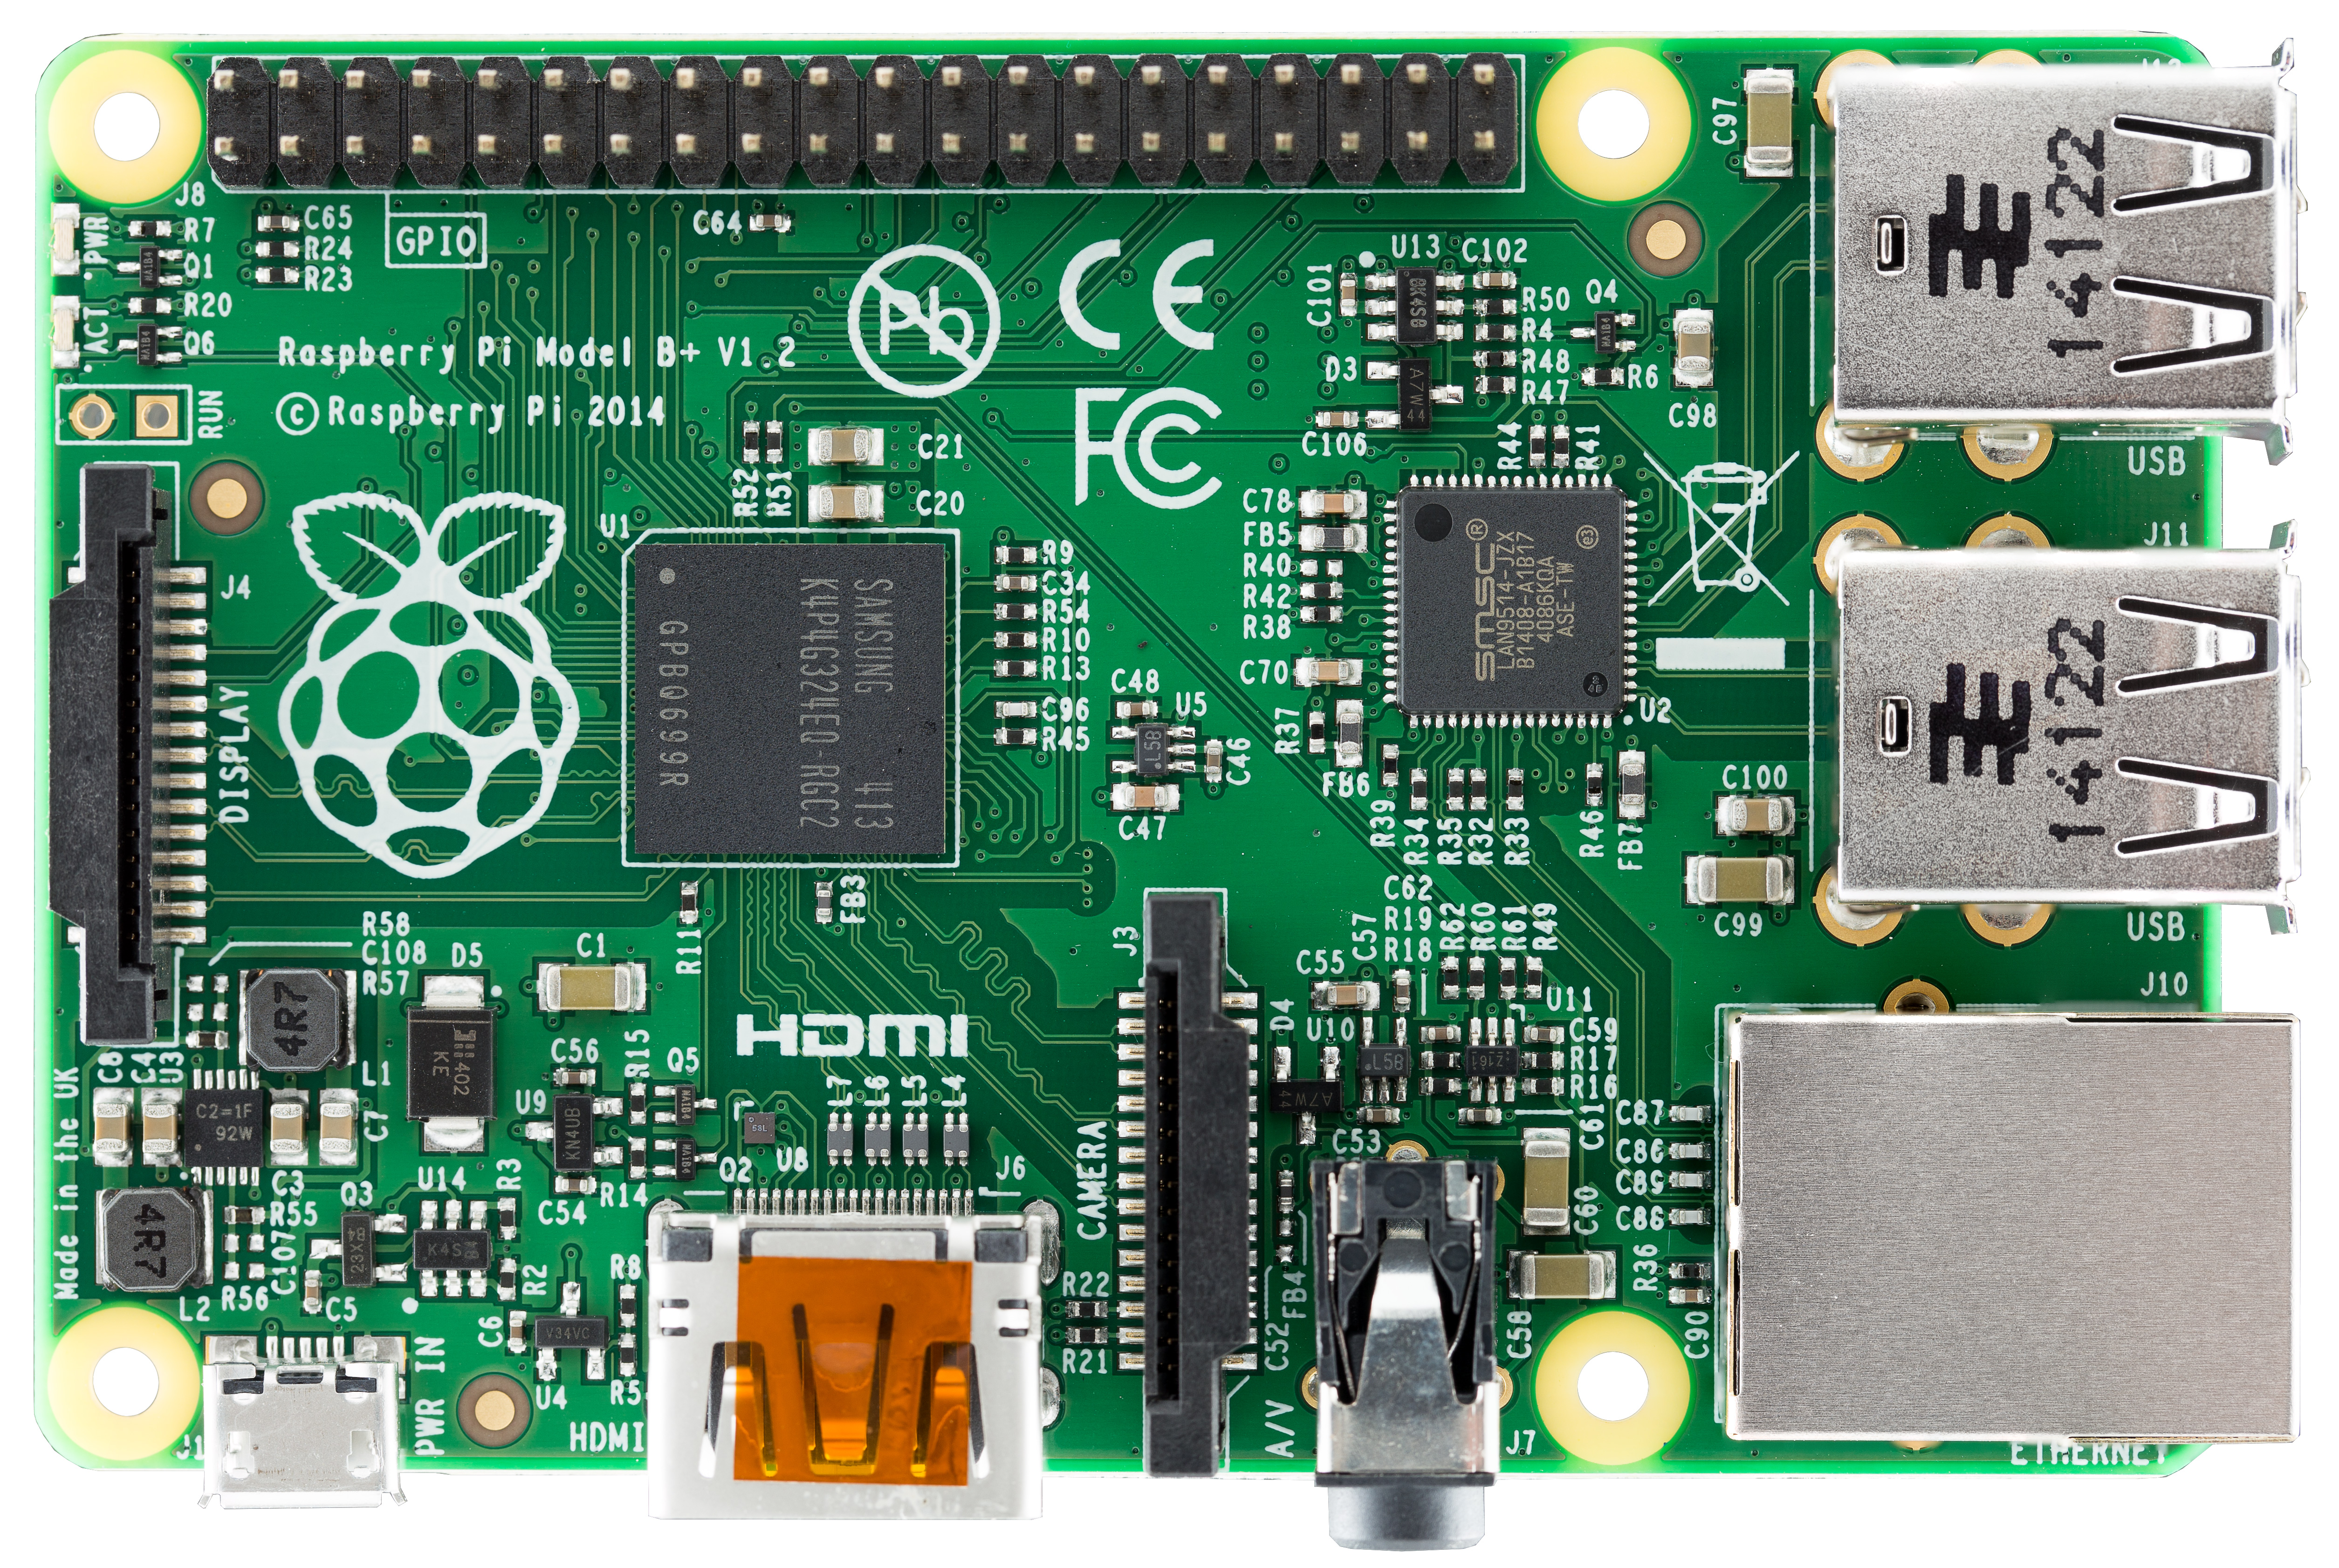
\includegraphics[scale=.085]{Raspberry_Pi_B+_top.jpg}
	
		\pagebreak

	\section{Definitions}
	
	\begin{itemize}
		\item Central Processing Unit (CPU):
		The part of a computer that is responsible for computations and executing commands. Frequently referred to as the brains of the computer.
		\item Register:
		Memory that is stored on the CPU that is ready to be executed or in process of being executed
		\item Bit:
		The most basic unit of storage in machine language, can only hold a value of Charged or not charged, 1 or 0, TRUE or FALSE
		\item Byte:
		A collection of 8 bits into a single unit.
		\item Halfword:
		A collection of 16 bits (According to ARM Documentation A2.2)  
		[NOTE: This is very different from x86 architecture. A Word is 16 bits in x86.]
		\item Word:
		A collection of 32 bits
		\item Doubleword:
		A collection of 64 bits (this is possible even though it is running on a 32 bit processor)
		\item Most Significant Bit:
		The largest Bit in a series of bits.  
		Reading this series of numbers the 1 will be the Most Significant Bit, 1000
		\item Big Endian:
		A method of storing data form MSB (Most significant byte) to LSB (Least significant byte).  
		\item Little Endian:
		A method of storing data from LSB to MSB. (This is the most common today)
		\item Bi-Endian:
		Being able to read either Big or Little Endian. 
		\item RISC:
		Reduced Instruction Set Computer
		
	\end{itemize}
	
	\section{History}
	
	\noindent \tiny{For the purposes of this paper I will be using ARMv6, ARM11, and ARM interchangeably from here on out.}
	
	\noindent \normalsize{What does ARM stand for?
	ARM stands for \textit{Advanced RISC Machine}. At least that's what it means now; it originally stood for \textit{Acorn RISC Machine} because \textit{Acorn Computers LDT}. was the company that created ARM. Acorn was a British company based out of Cambridge and has since changed to \textit{Element14} in the late 1990's.  
	Apple briefly helped develop with ARM creating what would eventually be called the ARM6. Legal entanglements with Intel would have that architecture help developing Intel's StrongARM processor. Intel would later invent their own RISC processor.}

	\pagebreak
	
	\section{Instruction Set}
	
	The ARM11 processor family actually use two instruction sets, 32-bit ARM and 16-bit Thumb (for the purpose of this paper I will focus on the 32-bit instruction set). ARM uses the same registers for the first 8 registers in all of their architectures, R0-R7.
	
	\begin{center}
		\begin{tabular}{ c c c}
			Register Number & Register Name & Register Type \\
			\hline
			1     	        & R0       		&  General Purpose  \\
			2               & R1       &  General Purpose  \\
			3               & R2       &  General Purpose  \\
			4               & R3       &  General Purpose  \\
			5               & R4       &  General Purpose  \\
			6               & R5       &  General Purpose  \\
			7               & R6       &  General Purpose  \\
			8               & R7       &  General Purpose  \\
			9               & R8       &  General Purpose  \\
			10              & R9       &  General Purpose  \\
			11              & R10      &  General Purpose  \\
			12              & R11      &  General Purpose  \\
			13              & R12      &  General Purpose  \\
			14              & SP\_main  &  Stack Pointer    \\
			15              & SP\_process &  Stack Pointer  \\
			16              & LR       & Link Register     \\
			17              & PC       & Program Counter   \\
			18              & APSR     & Special-purpose Program Status Register    \\
			19              & IPSR     & Special-purpose Program Status Register  \\
			20              & SPSR     & Special-purpose Program Status Register    \\
			21              & PRIMASK  & Special-purpose mask register   \\
			22              & CONTROL  & Special-Purpose Control register    \\
			
		\end{tabular}
	\end{center}
	
	\section{Instructions}
	
	\noindent
	ARM instructions work very different from x86 architecture in that from many commands the destination can be a location completely different than one of the operands. A quick example of this could be the add operation:  
	x86 (NASM):
	
	\begin{code}
		ADD eax, ebx   
	\end{code}  
	
	\noindent
	This takes the values in registers eax and ebx adds them and stores them in eax.
	
	\noindent
	Where in ARM:
	
	
	\begin{code}
		ADD R0, R1, R2
	\end{code}
	
	\noindent
	takes the values in R1 and R2, adds them, then stores them in R0.  
	It is important to remember when running these operations that data must be moved to a register before it can be manipulated.
	
	\begin{center}
		\begin{tabular}{ c c c }
			
			Mnemonic       & Instruction              & Comments      \\
			\hline
			ADC            & Add with carry           & \\
			ADD            & Add                      & \\
			ADR            & Form PC-relative Address & The first operand is PC and second is an immediate constant. \\
			AND            & Bitwise And              & \\
			BIC            & Bitwise Clear            & \\
			CMN            &Compare Negative         & Sets the flags as if addition was preformed but does not store the value \\
			CMP            & Compare                  & Sets the flags as if subtraction was preformed but does not store the value \\
			EOR            & Bitwise Exclusive OR     & \\
			MOV            & Copies operand to destination & \\
			MVN            & Bitwise NOT              & Does not support immediate values \\
			ORR            & Bitwise OR               & \\
			RSB            & Revers subtraction       & subtracts the first operand from the second. \\
			SBC            & subtraction with carry   & \\
			TST            & Test                     & Sets flags as if AND was preformed but does not store the values \\
		\end{tabular}
	\end{center}		
	
	\section{Pipeline}
	
	ARM has an eight stage pipeline.
	
	\begin{center}
		\begin{tabular}{ c c }
			
			Mnemonic  & Description \\
			\hline
			Fe1       & Address is sent and instruction received \\
			Fe2       & Much of the branch prediction goes here    \\
			De        & Decode instruction  \\
			Iss       & Read register and issue instruction \\
			Sh        & Preform shift operation \\
			ALU       & Preform integer operations \\
			Sat       & Saturate results \\
			WB        & Write back data to registers \\
		\end{tabular}
	\end{center}
	
	\section{Memory Hierarchy}
	
	ARM11 has 5 levels in its memory hierarchy.  
	The levels from closest to CPU to Furthest are as follows:  
	\begin{itemize}
		\item CPU / registers 
		\item Level 1 Cache for instructions and data 
		\item Level 2 Cache 
		\item Virtual/physical pages in primary memory 
		\item Virtual pages in secondary storage.  
	\end{itemize} 
	
	\noindent
	As you get further and further from the CPU the time it takes to access the memory increases.
	
	\section{Memory Access}
	As I have stated in the \textit{Instructions section}, you cannot manipulate data unless it is in a register.
	
	\section{Resources}
	
	\noindent
	A list of tools and resources I used.
	
	\begin{itemize}
		
		\item \url{http://www.cs.virginia.edu/~skadron/cs433_s09_processors/arm11.pdf}
		
		\item \url{ARM.Reference_Manual_2.pdf}  
		
		\item \url{http://sandsoftwaresound.net/raspberry-pi/raspberry-pi-gen-1/memory-hierarchy/}
		
		\item \url{http://www.peter-cockerell.net/aalp/html/frames.html}
		
		\item \url{https://en.wikipedia.org/wiki/ARM11#/media/File:Raspberry_Pi_B%2B_top.jpg}
		
	\end{itemize}
	
\end{document}